\documentclass[aspectratio=169,10pt]{beamer}
\usetheme{Madrid}
\usepackage[T1]{fontenc}
\usepackage{lmodern}
\usepackage{tikz}
\usepackage{adjustbox}
\usetikzlibrary{arrows.meta,positioning,fit,backgrounds,calc,shadows,shapes.geometric}

% Brand Color Palette matching PrismSpace theme
\definecolor{prismNavy}{RGB}{13,29,54}
\definecolor{prismBlue}{RGB}{38,126,190}
\definecolor{prismTeal}{RGB}{28,161,157}
\definecolor{prismMint}{RGB}{232,248,245}
\definecolor{prismGold}{RGB}{229,166,50}
\definecolor{prismDark}{RGB}{15,23,42}
\definecolor{prismIndigo}{RGB}{79,70,229}
\definecolor{prismSlate}{RGB}{71,85,105}
\definecolor{cardBg}{RGB}{248,250,252}

% Harmonious pastel node fills
\definecolor{cInput}{RGB}{243,244,246}
\definecolor{cStem}{RGB}{224,231,255}
\definecolor{cStage1}{RGB}{220,252,231}
\definecolor{cStage2}{RGB}{254,243,199}
\definecolor{cStage3}{RGB}{254,226,226}
\definecolor{cStage4}{RGB}{224,242,254}
\definecolor{cHead}{RGB}{243,232,255}
\definecolor{cOutput}{RGB}{252,231,243}

\setbeamercolor{frametitle}{bg=prismNavy,fg=white}
\setbeamertemplate{navigation symbols}{}
\setbeamertemplate{footline}{\hfill\textbf{PrismSpace} $\cdot$ CSE, CEK\hspace{1em}|\hspace{1em}\insertframenumber/\inserttotalframenumber\hspace{1.5em}\vspace{0.4em}}

\begin{document}

\begin{frame}[t]{02. System Architecture: 6-Tier Stack \& Multi-Agent Workflow}
\vspace{-0.4em}
\centering
\adjustbox{max width=0.98\linewidth, max height=0.82\textheight}{%
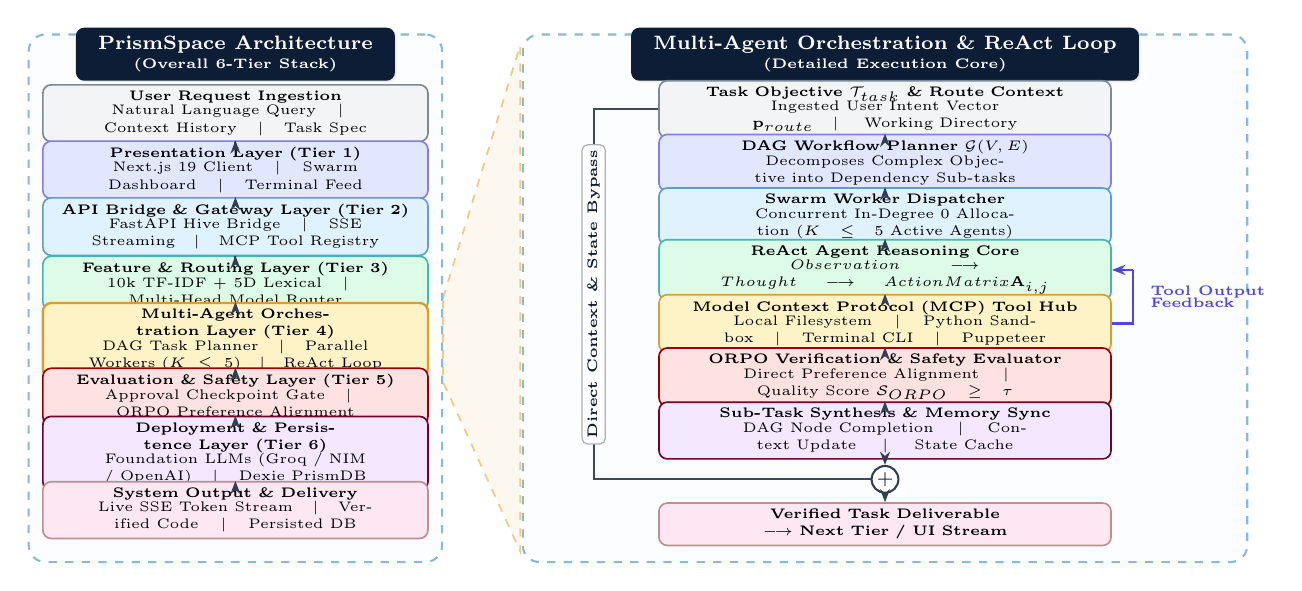
\begin{tikzpicture}[
  x=1cm, y=1cm,
  every node/.style={align=center},
  card/.style={
    draw=prismBlue!55, dashed, line width=0.75pt, fill=prismBlue!1.5,
    rounded corners=6pt
  },
  pilltitle/.style={
    fill=prismNavy, text=white, font=\scriptsize\bfseries,
    rounded corners=3pt, inner xsep=8pt, inner ysep=3.2pt,
    drop shadow={opacity=0.15, shadow xshift=0.5pt, shadow yshift=-0.5pt}
  },
  layerbox/.style={
    rectangle, rounded corners=3pt, line width=0.6pt,
    text width=4.75cm, minimum height=0.45cm, inner ysep=2.2pt, inner xsep=2pt,
    font=\fontsize{5.2}{6.2}\selectfont
  },
  detailbox/.style={
    rectangle, rounded corners=3pt, line width=0.6pt,
    text width=5.6cm, minimum height=0.45cm, inner ysep=2.2pt, inner xsep=2pt,
    font=\fontsize{5.2}{6.2}\selectfont
  },
  arrow/.style={
    -{Stealth[scale=0.75]}, line width=0.75pt, draw=prismNavy!85
  },
  conn/.style={
    draw=prismNavy!80, line width=0.75pt
  },
  plusnode/.style={
    circle, draw=prismNavy!85, line width=0.75pt, fill=white,
    inner sep=0pt, minimum size=0.34cm, font=\scriptsize\bfseries, text=prismNavy
  }
]

  % =========================================================================
  % LEFT CONTAINER: OVERALL 6-TIER ARCHITECTURE
  % Card 1: center=(2.85, 3.25), width=5.25cm, height=6.70cm => x in [0.22, 5.48]
  % =========================================================================
  \node[card, minimum width=5.25cm, minimum height=6.70cm] (card1) at (2.85, 3.25) {};
  \node[pilltitle] (title1) at (2.85, 6.35) {PrismSpace Architecture\\[-0.15em]{\fontsize{4.8}{5.8}\selectfont (Overall 6-Tier Stack)}};

  \node[layerbox, fill=cInput, draw=prismSlate!70] (l0) at (2.85, 5.60) {
    \textbf{User Request Ingestion}\\[-0.15em]
    \fontsize{4.5}{5.5}\selectfont Natural Language Query $\;\vert\;$ Context History $\;\vert\;$ Task Spec
  };

  \node[layerbox, fill=cStem, draw=prismIndigo!70] (l1) at (2.85, 4.88) {
    \textbf{Presentation Layer (Tier 1)}\\[-0.15em]
    \fontsize{4.5}{5.5}\selectfont Next.js 19 Client $\;\vert\;$ Swarm Dashboard $\;\vert\;$ Terminal Feed
  };

  \node[layerbox, fill=cStage4, draw=prismBlue!75] (l2) at (2.85, 4.16) {
    \textbf{API Bridge \& Gateway Layer (Tier 2)}\\[-0.15em]
    \fontsize{4.5}{5.5}\selectfont FastAPI Hive Bridge $\;\vert\;$ SSE Streaming $\;\vert\;$ MCP Tool Registry
  };

  \node[layerbox, fill=cStage1, draw=prismTeal!80] (l3) at (2.85, 3.44) {
    \textbf{Feature \& Routing Layer (Tier 3)}\\[-0.15em]
    \fontsize{4.5}{5.5}\selectfont 10k TF-IDF + 5D Lexical $\;\vert\;$ Multi-Head Model Router
  };

  \node[layerbox, fill=cStage2, draw=prismGold!95!black, line width=0.85pt] (l4) at (2.85, 2.72) {
    \textbf{Multi-Agent Orchestration Layer (Tier 4)}\\[-0.15em]
    \fontsize{4.5}{5.5}\selectfont DAG Task Planner $\;\vert\;$ Parallel Workers ($K \le 5$) $\;\vert\;$ ReAct Loop
  };

  \node[layerbox, fill=cStage3, draw=red!60!black] (l5) at (2.85, 2.00) {
    \textbf{Evaluation \& Safety Layer (Tier 5)}\\[-0.15em]
    \fontsize{4.5}{5.5}\selectfont Approval Checkpoint Gate $\;\vert\;$ ORPO Preference Alignment
  };

  \node[layerbox, fill=cHead, draw=purple!60!black] (l6) at (2.85, 1.28) {
    \textbf{Deployment \& Persistence Layer (Tier 6)}\\[-0.15em]
    \fontsize{4.5}{5.5}\selectfont Foundation LLMs (Groq / NIM / OpenAI) $\;\vert\;$ Dexie PrismDB
  };

  \node[layerbox, fill=cOutput, draw=pink!75!black] (l7) at (2.85, 0.56) {
    \textbf{System Output \& Delivery}\\[-0.15em]
    \fontsize{4.5}{5.5}\selectfont Live SSE Token Stream $\;\vert\;$ Verified Code $\;\vert\;$ Persisted DB
  };

  % Downward arrows on Left Card
  \draw[arrow] (l0) -- (l1);
  \draw[arrow] (l1) -- (l2);
  \draw[arrow] (l2) -- (l3);
  \draw[arrow] (l3) -- (l4);
  \draw[arrow] (l4) -- (l5);
  \draw[arrow] (l5) -- (l6);
  \draw[arrow] (l6) -- (l7);

  % =========================================================================
  % RIGHT CONTAINER: DETAILED VIEW (MULTI-AGENT ORCHESTRATION & REACT LOOP)
  % Card 2: center=(11.10, 3.25), width=9.20cm, height=6.70cm => x in [6.50, 15.70]
  % Gap between Card 1 & Card 2: [5.48, 6.50] = 1.02cm
  % Boxes centered at x=11.10, width=5.60cm => x in [8.30, 13.90]
  % Left corridor: [6.50, 8.30] = 1.80cm (Bypass line at x=7.40)
  % Right corridor: [13.90, 15.70] = 1.80cm (Feedback line at x=14.80)
  % =========================================================================
  \node[card, minimum width=9.20cm, minimum height=6.70cm] (card2) at (11.10, 3.25) {};
  \node[pilltitle] (title2) at (11.10, 6.35) {Multi-Agent Orchestration \& ReAct Loop\\[-0.15em]{\fontsize{4.8}{5.8}\selectfont (Detailed Execution Core)}};

  \node[detailbox, fill=cInput, draw=prismSlate!70] (d_in) at (11.10, 5.65) {
    \textbf{Task Objective $\mathcal{T}_{\text{task}}$ \& Route Context}\\[-0.15em]
    \fontsize{4.5}{5.5}\selectfont Ingested User Intent Vector $\mathbf{p}_{\text{route}} \;\vert\;$ Working Directory
  };

  \node[detailbox, fill=cStem, draw=prismIndigo!70] (d_plan) at (11.10, 4.97) {
    \textbf{DAG Workflow Planner $\mathcal{G}(V, E)$}\\[-0.15em]
    \fontsize{4.5}{5.5}\selectfont Decomposes Complex Objective into Dependency Sub-tasks
  };

  \node[detailbox, fill=cStage4, draw=prismBlue!75] (d_disp) at (11.10, 4.29) {
    \textbf{Swarm Worker Dispatcher}\\[-0.15em]
    \fontsize{4.5}{5.5}\selectfont Concurrent In-Degree 0 Allocation ($K \le 5$ Active Agents)
  };

  \node[detailbox, fill=cStage1, draw=prismTeal!80] (d_react) at (11.10, 3.61) {
    \textbf{ReAct Agent Reasoning Core}\\[-0.15em]
    \fontsize{4.5}{5.5}\selectfont $\text{Observation} \;\longrightarrow\; \text{Thought} \;\longrightarrow\; \text{Action Matrix } \mathbf{A}_{i,j}$
  };

  \node[detailbox, fill=cStage2, draw=prismGold!95!black] (d_mcp) at (11.10, 2.93) {
    \textbf{Model Context Protocol (MCP) Tool Hub}\\[-0.15em]
    \fontsize{4.5}{5.5}\selectfont Local Filesystem $\;\vert\;$ Python Sandbox $\;\vert\;$ Terminal CLI $\;\vert\;$ Puppeteer
  };

  \node[detailbox, fill=cStage3, draw=red!60!black] (d_eval) at (11.10, 2.25) {
    \textbf{ORPO Verification \& Safety Evaluator}\\[-0.15em]
    \fontsize{4.5}{5.5}\selectfont Direct Preference Alignment $\;\vert\;$ Quality Score $\mathcal{S}_{\text{ORPO}} \ge \tau$
  };

  \node[detailbox, fill=cHead, draw=purple!60!black] (d_agg) at (11.10, 1.57) {
    \textbf{Sub-Task Synthesis \& Memory Sync}\\[-0.15em]
    \fontsize{4.5}{5.5}\selectfont DAG Node Completion $\;\vert\;$ Context Update $\;\vert\;$ State Cache
  };

  \node[plusnode] (plus) at (11.10, 0.95) {$+$};

  \node[detailbox, fill=cOutput, draw=pink!75!black] (d_out) at (11.10, 0.38) {
    \textbf{Verified Task Deliverable $\longrightarrow$ Next Tier / UI Stream}
  };

  % Downward arrows on Right Card
  \draw[arrow] (d_in) -- (d_plan);
  \draw[arrow] (d_plan) -- (d_disp);
  \draw[arrow] (d_disp) -- (d_react);
  \draw[arrow] (d_react) -- (d_mcp);
  \draw[arrow] (d_mcp) -- (d_eval);
  \draw[arrow] (d_eval) -- (d_agg);
  \draw[arrow] (d_agg) -- (plus);
  \draw[arrow] (plus) -- (d_out);

  % =========================================================================
  % RESIDUAL / ITERATIVE FEEDBACK LOOP (LEFT & RIGHT CORRIDORS OF RIGHT CARD)
  % =========================================================================
  % Direct Context & State Bypass (Left corridor at x=7.40, completely clear)
  \draw[conn] (d_in.west) -- (7.40, 5.65) -- (7.40, 0.95) -- (plus.west);
  \node[font=\fontsize{4.6}{5.6}\selectfont\bfseries, text=prismNavy, fill=white, draw=prismNavy!35, line width=0.45pt, rounded corners=2pt, inner sep=2pt] 
    at (7.40, 3.30) [rotate=90] {Direct Context \& State Bypass};

  % Iterative ReAct tool feedback loop (Right corridor: clear bracket + readable label)
  \draw[conn, draw=prismIndigo, line width=0.8pt] (d_mcp.east) -- (14.25, 2.93) -- (14.25, 3.61);
  \draw[arrow, draw=prismIndigo, line width=0.8pt] (14.25, 3.61) -- (d_react.east);
  \node[font=\fontsize{4.4}{5.2}\selectfont\bfseries, text=prismIndigo, align=left, anchor=west]
    at (14.35, 3.27) {Tool Output\\[-0.15em]Feedback};

  % =========================================================================
  % CLEAN ZOOM PROJECTION BEAM FROM TIER 4 (Strictly between cards, on background)
  % =========================================================================
  \begin{scope}[on background layer]
    \fill[prismGold!8, draw=prismGold!60, dashed, line width=0.65pt] 
      ($(card1.east |- l4.north)+(0, 0.05)$) -- 
      ($(card2.west |- card2.north)+(-0.02, -0.15)$) -- 
      ($(card2.west |- card2.south)+(-0.02, 0.15)$) -- 
      ($(card1.east |- l4.south)+(0, -0.05)$) -- cycle;
    \draw[prismGold!80!black, line width=0.85pt] (l4.north east) -- ($(card1.east |- l4.north)+(0, 0.05)$);
    \draw[prismGold!80!black, line width=0.85pt] (l4.south east) -- ($(card1.east |- l4.south)+(0, -0.05)$);
  \end{scope}

\end{tikzpicture}%
}
\end{frame}

\end{document}
